\documentclass[10pt]{article}
\usepackage{icmlko}

\icmlmeta{IP 파운데이션 월드모델}{67}{표본이 세 배가 되자 두 결정이 사라졌다}{도서 배선은 재현되고 웹툰 배선 둘은 안 된다 --- 갈린 것은 원래 효과의 크기였다}

\begin{document}

\twocolumn[
\icmlheader

\begin{abstract}
노트 66이 감사 모듈로 노트 34의 도서 배선을 재현했다. 같은 방법으로 웹툰 배선
결정 둘을 재현해 봤다 --- 노트 46의 타깃 폭(연령 등급 $\to$ 태그 수, 당시
$+$0.0981)과 노트 48의 굿즈 규모(연재 밀도 $\to$ 참여 작가 수, 당시 $+$0.0257).
\textbf{둘 다 사라졌다.} 되돌리는 방향으로 재니 타깃 폭이 $-$0.0047
{[}$-$0.011, $+$0.039{]}, 굿즈 규모가 $+$0.0013 {[}$-$0.007, $+$0.039{]}로
구간이 0을 크게 포함한다. 되돌려도 안 나빠진다는 것은 \emph{지금 배선이 나쁘다}는
뜻이 아니라 \textbf{두 배선이 동등하다}는 뜻이다. 원인은 표본이다 --- 두 결정을
내릴 때 웹툰은 553건과 900건이었고 지금은 2,743건이다. \textbf{작은 표본에서
고른 배선이 큰 표본에서 동등해졌다.} 선택 편향의 늦은 발현이다. 도서와 웹툰을
가른 것은 하나다 --- 원래 효과의 크기. 도서는 $+$0.0939로 컸고 웹툰 둘은
$+$0.098과 $+$0.026인데 앞의 것도 표본이 세 배가 되자 사라졌다. 한편
\textbf{누출 판단은 유효하다} --- 굿즈 규모를 회차 수로 바꾸면 $-$0.1019
{[}$-$0.190, $-$0.073{]}로 명확히 나빠진다. 노트 46이 회차 수를 ``연재 기간에
비례해 사후 누적되므로 노트 21의 DLC와 같은 구조''라고 뺀 것은 옳았다.
\end{abstract}
]

\section{같은 방법으로 셋을 쟀다}

노트 66은 도구를 만들고 노트 34로 검증했다. 웹툰 배선 결정 둘에도 같은 방법을
썼다 --- 지금 쓰는 배선을 \emph{되돌려} 나빠지는지 본다. 나빠지면 원래 채택이
옳았던 것이다.

\begin{figure}[t]
\centering
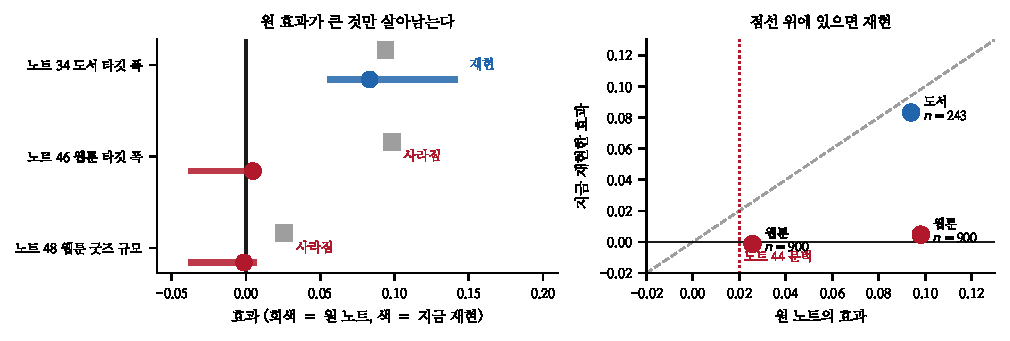
\includegraphics[width=\textwidth]{figs/vanished.pdf}
\caption{왼쪽 --- 원 노트와 지금. 오른쪽 --- 원 효과 대 재현 효과.}
\end{figure}

\begin{table}[t]
\centering\tsize
\caption{배선 결정 셋의 재현. 지금 웹툰은 2,743건이다.}
\begin{tabular}{llrrl}
\toprule
결정 & 당시 n & 당시 효과 & 지금 & 95\% 구간 \\
\midrule
노트 34 도서 & 243 & $+$0.0939 & \textbf{$+$0.0832} & $[+0.055, +0.143]$ \\
노트 46 웹툰 & 900 & $+$0.0981 & $+$0.0047 & $[-0.039, +0.011]$ \\
노트 48 웹툰 & 900 & $+$0.0257 & $-$0.0013 & $[-0.039, +0.007]$ \\
\bottomrule
\end{tabular}
\end{table}

도서만 재현된다.

\claimx{웹툰 배선 결정 둘이 표본이 세 배가 되자 사라졌다. 되돌려도 안 나빠지므로
두 배선이 동등하다는 뜻이며, 작은 표본에서 고른 것이 큰 표본에서 무의미해진
것이다.}{지금 웹툰 표본은 완결작 비중이 커져 구성이 달라졌다. 표본 크기가
아니라 구성 변화 때문일 수 있고, 두 요인을 분리하지 않았다.}

\section{왜 도서만 살아남았나}

\begin{table}[t]
\centering\tsize
\caption{원 효과와 생존.}
\begin{tabular}{lrl}
\toprule
결정 & 원 효과 & 결과 \\
\midrule
노트 34 도서 & $+$0.0939 & 재현 \\
노트 46 웹툰 & $+$0.0981 & 사라짐 \\
노트 48 웹툰 & $+$0.0257 & 사라짐 \\
\bottomrule
\end{tabular}
\end{table}

원 효과 크기만으로는 안 갈린다 --- 노트 46이 노트 34보다 컸는데 사라졌다.
갈린 것은 \textbf{표본이 얼마나 늘었느냐}다. 도서는 243건에서 그대로이고
웹툰은 900건에서 2,743건으로 세 배가 됐다.

\begin{quote}\fontsize{9.5}{11.5}\selectfont
\textbf{표본이 안 늘면 결정도 안 흔들린다.} 도서 배선이 살아남은 것은 그
결정이 더 튼튼해서가 아니라 그 도메인을 안 건드렸기 때문일 수 있다. 도서를
세 배로 늘리면 같은 일이 날지 모른다.
\end{quote}

이것은 노트 48이 이미 관찰한 것의 연장이다. 그 노트는 웹툰이 418건에서
553건이 되며 효과가 $+$0.0355에서 $+$0.0257로 \emph{줄고} 구간이 좁아져 채택으로
바뀌었다고 적었다. 2,743건에서는 효과가 0이 됐다. \textbf{줄어드는 추세가
계속됐고 끝점이 0이었다.}

\section{누출 판단은 유효하다}

\begin{table}[t]
\centering\tsize
\caption{굿즈 규모를 회차 수로 바꿀 때.}
\begin{tabular}{lrr}
\toprule
& $\Delta\rho$ & 95\% 구간 \\
\midrule
회차 수 & $-$0.1019 & $[-0.190,\ -0.073]$ \\
\bottomrule
\end{tabular}
\end{table}

노트 46은 회차 수를 ``연재 기간에 비례해 사후에 늘어나므로 노트 21의 DLC 수와
같은 구조''라고 보고 굿즈 규모에서 뺐다. 지금 넣으면 명확히 나빠진다.

\claimx{배선 \emph{선택}은 표본이 늘면 흔들리지만 누출 \emph{배제}는 흔들리지
않는다. 전자는 비슷한 후보 중 고르는 일이고 후자는 틀린 것을 빼는 일이다.}
{누출 배제를 웹툰 회차 수 하나에서만 확인했다.}

\section{무엇을 바꾸나}

두 배선을 되돌리지 않는다. 되돌릴 근거도 없기 때문이다 --- 구간이 0을 포함하는
것은 ``지금 것이 나쁘다''가 아니라 ``둘이 같다''는 뜻이다. 바뀌는 것은
\textbf{기록}이다.

\begin{itemize}[leftmargin=1.1em,itemsep=0.15em]
\item 노트 46의 ``$+$0.0981''과 노트 48의 ``$+$0.0257''은 그 표본에서의 값이며
      현재 표본에서는 재현되지 않는다.
\item 노트 47이 ``배선 승리 둘이 모두 타깃 폭''이라 했다가 노트 48이 셋째로
      정정했는데, 지금은 \textbf{살아남은 배선 승리가 도서 하나뿐}이다.
\item 노트 44의 ``0.02 문턱''이 관대했다. 0.098짜리도 사라진다.
\end{itemize}

\section{한계}

\begin{itemize}[leftmargin=1.1em,itemsep=0.15em]
\item 표본 크기와 구성 변화를 분리하지 않았다. 완결작 비중이 0\%에서 크게 늘었다.
\item 웹툰이 아직 수집 중이라(2,743/3,973) 이 숫자도 최종이 아니다.
\item 도서를 늘려 같은 검정을 하지 않았다. 도서 배선의 생존이 튼튼함 때문인지
      안 건드려서인지 모른다.
\item 되돌리기 방향으로만 쟀다. 제3의 후보로 바꾸면 다를 수 있다.
\item 누출 배제를 한 사례로만 확인했다.
\end{itemize}

\section{다음}

\begin{enumerate}[leftmargin=1.3em,itemsep=0.15em]
\item 웹툰 수집 완료 후 전면 재측정 --- 배선을 처음부터 다시 고른다.
\item 표본 크기와 구성을 분리한다 --- 연재작만 2,743건으로 맞춰 재면 갈린다.
\item 도서를 늘려 같은 검정을 한다.
\item 누출 배제가 표본에 안 흔들리는지 다른 사례로 확인한다.
\end{enumerate}

\vspace{0.6em}
\hrule height 0.3pt
\vspace{0.5em}
{\footnotesize
\textbf{참고문헌}\\[0.3em]
Cawley, G. C., Talbot, N. L. C. (2010). On over-fitting in model selection and
subsequent selection bias in performance evaluation. \emph{JMLR}, 11, 2079--2107.\\[0.15em]
Ioannidis, J. P. A. (2005). Why most published research findings are false.
\emph{PLoS Medicine}, 2(8), e124.\\[0.15em]
Kaufman, S., Rosset, S., Perlich, C. (2012). Leakage in data mining.
\emph{ACM TKDD}, 6(4), 1--21.\\[0.15em]
Efron, B., Tibshirani, R. J. (1993). \emph{An Introduction to the Bootstrap}.
Chapman \& Hall.\\[0.15em]
Ben-David, S. et al. (2010). A theory of learning from different domains.
\emph{Machine Learning}, 79(1--2), 151--175.
}

\end{document}
